\providecommand{\main}{../..}%define path to bib for subfiles
\documentclass[../../main.tex]{subfiles}
\begin{document}
\onlyinsubfile{\setcounter{chapter}{8}}
\notinsubfile{}
\chapter{Cheatsheet}
wordt tabel op een enkelzijdige pagina. enkelvoudige poorten en CNOT apart

tensorvermenigvuldiging

\onlyinsubfile{
\marginpar{\vspace{0cm}
\textcolor{red}{hoofdstuk is los gecompileerd, hstk nummer is \thechapter}
}
}
\notinsubfile{
\marginpar{\vspace{0cm}
\textcolor{red}{main.tex gecompileerd, nummering zou moeten kloppen}}
}

\subsection{De I-poort}
\begin{center}
\leavevmode
\begin{figure}[h]
\begin{subfigure}[b]{.3\textwidth}
\begin{center}
$I=\mqty(1&0\\0&1)$
\end{center}
\vspace{.5cm}
  \caption{matrix}
%  \label{fig:sub1}
\end{subfigure}%
\begin{subfigure}[b]{.3\textwidth}
\hspace{1cm}
\Qcircuit @C=1em @R=2em {
%\ustick{\ket{0}}
& \gate{I} & \qw & \\
}
\vspace{1cm}
  \caption{circuit}
%  \label{fig:sub2}
\end{subfigure}
\begin{subfigure}[b]{.3\textwidth}
\begin{center}
\begin{tikzpicture}[>=stealth]
\matrix (A) [matrix of nodes,row sep=3mm,column sep=3mm,nodes in empty cells]
{
$\ket{0}$   & & & $\ket{0}$\\
$\ket{1}$   & & & $\ket{1}$\\
};
\begin{scope}[thick,red,<->]
\draw (A-1-1)--(A-1-4);
\draw (A-2-1)--(A-2-4);
\end{scope}
\end{tikzpicture}
\end{center}
  \caption{afbeelding}
%  \label{fig:sub3}
\end{subfigure}
\caption{\port{I}-poort: matrix, circuit en afbeelding van basisvectoren}
\label{fig:ipoort}
\end{figure}
\end{center}

\section{De X-poort}
\begin{center}
\leavevmode
\begin{figure}[h]
\begin{subfigure}[b]{.3\textwidth}
\begin{center}
$ X=\mqty(0&1\\1&0)$
\end{center}
\vspace{.5cm}
  \caption{matrix}
%  \label{fig:sub1}
\end{subfigure}%
\begin{subfigure}[b]{.3\textwidth}
\hspace{1cm}
\Qcircuit @C=1em @R=2em {
%\ustick{\ket{0}}
& \gate{X} & \qw & \\
}
\vspace{1cm}
  \caption{circuit}
%  \label{fig:sub2}
\end{subfigure}
\begin{subfigure}[b]{.3\textwidth}
\begin{center}
\begin{tikzpicture}[>=stealth]
\matrix (A) [matrix of nodes,row sep=3mm,column sep=3mm,nodes in empty cells]
{
$\ket{0}$   & & & $\ket{1}$\\
$\ket{1}$   & & & $\ket{0}$\\
};
\begin{scope}[thick,red,<->]
\draw (A-1-1)--(A-1-4);
\draw (A-2-1)--(A-2-4);
\end{scope}
\end{tikzpicture}
\end{center}
  \caption{afbeelding}
%  \label{fig:sub3}
\end{subfigure}
\caption{\port{X}-poort: matrix, circuit en afbeelding van basisvectoren}
\label{fig:xpoort}
\end{figure}
\end{center}


$\mqty(\alpha\\\beta)\leftrightarrow\mqty(\beta\\\alpha)$

In fig.~\ref{fig:stateX} staat voor acht toestanden de werkingen van de X-poort uitgetekend. Is de X-poort omkeerbaar? Wat gebeurt er als je hem twee keer toepast?

\begin{center}
\leavevmode
\begin{tikzpicture}[scale=.5]
\def\vectsize{.7}
\def\radius{5cm}
\def\labelrad{4.cm}
\def\ketrad{5.9cm}
\def\arrowrad{3cm}
\draw (0,0) circle (\radius);
\foreach \x in {0,45,...,315} \filldraw (\x:\radius) circle (.1);

%\node[color=black, anchor=west] at (-2,8) {toestandsdiagram}; 
\node[color=green, anchor=west] at (-7,4.) {\footnotesize{X-poort}}; 

\node[scale=1] at ( 90:\ketrad) {$\ket{1}$};
\node[scale=1] at (  0:\ketrad) {$\ket{0}$};
%\node[scale=1] at (-90:\ketrad) {$\ket{1}$};
%\node[scale=1] at (180:\ketrad) {$\ket{0}$};
\node[scale=1] at ( 45:\ketrad) {$\ket{+}$};
%\node[scale=1] at (135:\ketrad) {$\ket{-}$};
%\node[scale=1] at (225:\ketrad) {$\ket{+}$};
\node[scale=1] at (-45:\ketrad) {$\ket{-}$};

%relaties X-gate
\draw[color=green, <->] (+90:\arrowrad) -- (0:\arrowrad);
\draw[color=green, <->] (+135:\arrowrad) -- (-45:\arrowrad);
\draw[color=green, <->] (+180:\arrowrad) -- (-90:\arrowrad);
\draw[color=green, <->] ( 4.3, 4.3)+(240:1.) arc (240:570:1.);
\draw[color=green, <->] (-4.3,-4.3)+( 60:1.) arc ( 60:390:1.);

\node[scale=\vectsize] at ( +90:\labelrad) {$\mqty( 0 \\ 1 )$};
\node[scale=\vectsize] at ( +45:\labelrad) {$
\mqty( \tfrac{1}{\sqrt{2}} \\ \tfrac{1}{\sqrt{2}} ) $};
\node[scale=\vectsize] at (   0:\labelrad) {$\mqty( 1 \\ 0 )$};
\node[scale=\vectsize] at ( -45:\labelrad) {$
\mqty( \tfrac{1}{\sqrt{2}}  \\ \tfrac{-1}{\sqrt{2}} ) $};
\node[scale=\vectsize] at ( -90:\labelrad) {$\mqty( 0 \\ -1 )$};
\node[scale=\vectsize] at (-135:\labelrad) {$
\mqty( \tfrac{-1}{\sqrt{2}}  \\ \tfrac{-1}{\sqrt{2}} ) $};
\node[scale=\vectsize] at ( 180:\labelrad) {$\mqty( -1\\ 0 )$};
\node[scale=\vectsize] at ( 135:\labelrad) {$
\mqty( \tfrac{-1}{\sqrt{2}}  \\ \tfrac{1}{\sqrt{2}} ) $};
\end{tikzpicture}
\captionof{figure}{toestandsdiagram voor \port{X}-poort. \label{fig:stateX}}
\end{center}


\section{De \port{Z}-poort}

\begin{center}
\leavevmode
\begin{figure}[h]
\begin{subfigure}[b]{.3\textwidth}
\begin{center}
$Z=\mqty(1&0\\0&-1)$
\end{center}
\vspace{.5cm}
  \caption{matrix}
%  \label{fig:sub1}
\end{subfigure}%
\begin{subfigure}[b]{.3\textwidth}
\hspace{1cm}
\Qcircuit @C=1em @R=2em {
%\ustick{\ket{0}}
& \gate{Z} & \qw & \\
}
\vspace{1cm}
  \caption{circuit}
%  \label{fig:sub2}
\end{subfigure}
\begin{subfigure}[b]{.3\textwidth}
\begin{center}
\begin{tikzpicture}[>=stealth]
\matrix (A) [matrix of nodes,row sep=3mm,column sep=3mm,nodes in empty cells]
{
$\ket{0}$   & & & $\ket{0}$\\
$\ket{1}$   & & & $\ket{-1}$\\
};
\begin{scope}[thick,red,<->]
\draw (A-1-1)--(A-1-4);
\draw (A-2-1)--(A-2-4);
\end{scope}
\end{tikzpicture}
\end{center}
  \caption{afbeelding}
%  \label{fig:sub3}
\end{subfigure}
\caption{\port{Z}-poort: matrix, circuit en afbeelding van basisvectoren}
\label{fig:zpoort}
\end{figure}
\end{center}

\begin{center}
\leavevmode
\begin{tikzpicture}[scale=.5]
\def\vectsize{.7}
\def\radius{5cm}
\def\labelrad{4.cm}
\def\ketrad{5.9cm}
\def\arrowrad{3cm}
\draw (0,0) circle (\radius);
\foreach \x in {0,45,...,315} \filldraw (\x:\radius) circle (.1);

%\node[color=black, anchor=west] at (-8,5) {toestandsdiagram van }; 
\node[color=blue,  anchor=west] at (-7,4.) {\footnotesize{Z-poort}}; 

\node[scale=1] at ( 90:\ketrad) {$\ket{1}$};
\node[scale=1] at (  0:\ketrad) {$\ket{0}$};
%\node[scale=1] at (-90:\ketrad) {$\ket{1}$};
%\node[scale=1] at (180:\ketrad) {$\ket{0}$};
\node[scale=1] at ( 45:\ketrad) {$\ket{+}$};
%\node[scale=1] at (135:\ketrad) {$\ket{-}$};
%\node[scale=1] at (225:\ketrad) {$\ket{+}$};
\node[scale=1] at (-45:\ketrad) {$\ket{-}$};

%relaties Z-gate
\draw[color=blue, <->] ( +45:\arrowrad) -- ( -45:\arrowrad);
\draw[color=blue, <->] ( +90:\arrowrad) -- ( -90:\arrowrad);
\draw[color=blue, <->] (+135:\arrowrad) -- (-135:\arrowrad);
\draw[color=blue, <->] ( 6.0, 0.0)+(195:1.) arc (195:525:1.);
\draw[color=blue, <->] (-6.0,-0.0)+( 15:1.) arc ( 15:345:1.);

\node[scale=\vectsize] at ( +90:\labelrad) {$\mqty( 0 \\ 1 )$};
\node[scale=\vectsize] at ( +45:\labelrad) {$
\mqty( \tfrac{1}{\sqrt{2}} \\ \tfrac{1}{\sqrt{2}} ) $};
\node[scale=\vectsize] at (   0:\labelrad) {$\mqty( 1 \\ 0 )$};
\node[scale=\vectsize] at ( -45:\labelrad) {$
\mqty( \tfrac{1}{\sqrt{2}}  \\ \tfrac{-1}{\sqrt{2}} ) $};
\node[scale=\vectsize] at ( -90:\labelrad) {$\mqty( 0 \\ -1 )$};
\node[scale=\vectsize] at (-135:\labelrad) {$
\mqty( \tfrac{-1}{\sqrt{2}}  \\ \tfrac{-1}{\sqrt{2}} ) $};
\node[scale=\vectsize] at ( 180:\labelrad) {$\mqty( -1\\ 0 )$};
\node[scale=\vectsize] at ( 135:\labelrad) {$
\mqty( \tfrac{-1}{\sqrt{2}}  \\ \tfrac{1}{\sqrt{2}} ) $};
\end{tikzpicture}
\captionof{figure}{Toestandsdiagram voor de \port{Z}-poort. \label{fig:stateZ}}
\end{center}


je ziet dat deze poort alleen in een quantumcomputer kan bestaan. De afbeelding op $\mqty(0\\-1)$
heeft pas betekenis na het kwadrateren van de co\"efficient ($\beta=-1$.

\section{De H-poort}
De Hadamard-poort transponeert de computational basis van en naar de Bell basis, een belangrijke stap in een quantumalgoritme.

\begin{center}
\leavevmode
\begin{figure}[h]
\begin{subfigure}[b]{.3\textwidth}
\begin{center}
$H=\frac{1}{\sqrt{2}}\mqty(1&1\\1&-1)$
\end{center}
\vspace{.5cm}
\caption{matrix}
%  \label{fig:sub1}
\end{subfigure}%
\begin{subfigure}[b]{.3\textwidth}
\hspace{1cm}
\Qcircuit @C=1em @R=2em {
%\ustick{\ket{0}}
& \gate{H} & \qw & \\
}
\vspace{1cm}
  \caption{circuit}
%  \label{fig:sub2}
\end{subfigure}
\begin{subfigure}[b]{.3\textwidth}
\begin{center}
\begin{tikzpicture}[>=stealth]
\matrix (A) [matrix of nodes,row sep=3mm,column sep=3mm,nodes in empty cells]
{
$\ket{0}$   & & & $\tfrac{1}{\sqrt{2}}(\ket{0}$+$\ket{1})=\ket{+}$\\
$\ket{1}$   & & & $\tfrac{1}{\sqrt{2}}(\ket{0}$-$\ket{1})=\ket{-}$\\
};
\begin{scope}[thick,red,<->]
\draw (A-1-1)--(A-1-4);
\draw (A-2-1)--(A-2-4);
\end{scope}
\end{tikzpicture}
\end{center}
  \caption{afbeelding}
%  \label{fig:sub3}
\end{subfigure}
\caption{\port{H}-poort: matrix, circuit en afbeelding van basisvectoren}
\label{fig:hpoort}
\end{figure}
\end{center}

Ook voor een Hadamard gate kun je een toestandsdiagram maken. 

\begin{center}
\leavevmode
\begin{tikzpicture}[scale=.5]
\def\vectsize{.7}
\def\radius{5cm}
\def\labelrad{4.cm}
\def\ketrad{5.9cm}
\def\arrowrad{3cm}
\draw (0,0) circle (\radius);
\foreach \x in {0,45,...,315} \filldraw (\x:\radius) circle (.1);

%\node[color=black, anchor=west] at (-7,5) {Toestandsdiagram}; 
\node[color=red,   anchor=west] at (-7,4) {\footnotesize{H-poort}}; 

\node[scale=1] at ( 90:\ketrad) {$\ket{1}$};
\node[scale=1] at (  0:\ketrad) {$\ket{0}$};
%\node[scale=1] at (-90:\ketrad) {$\ket{1}$};
%\node[scale=1] at (180:\ketrad) {$\ket{0}$};
\node[scale=1] at ( 45:\ketrad) {$\ket{+}$};
%\node[scale=1] at (135:\ketrad) {$\ket{-}$};
%\node[scale=1] at (225:\ketrad) {$\ket{+}$};
\node[scale=1] at (-45:\ketrad) {$\ket{-}$};

%relaties Hadamard
\draw[color=red, <->] ( +45:\arrowrad) -- (0:\arrowrad);
\draw[color=red, <->] ( +90:\arrowrad) -- (-45:\arrowrad);
\draw[color=red, <->] (+135:\arrowrad) -- (-90:\arrowrad);
\draw[color=red, <->] (+180:\arrowrad) -- (225:\arrowrad);

\node[scale=\vectsize] at ( +90:\labelrad) {$\mqty( 0 \\ 1 )$};
\node[scale=\vectsize] at ( +45:\labelrad) {$
\mqty( \tfrac{1}{\sqrt{2}} \\ \tfrac{1}{\sqrt{2}} ) $};
\node[scale=\vectsize] at (   0:\labelrad) {$\mqty( 1 \\ 0 )$};
\node[scale=\vectsize] at ( -45:\labelrad) {$
\mqty( \tfrac{1}{\sqrt{2}}  \\ \tfrac{-1}{\sqrt{2}} ) $};
\node[scale=\vectsize] at ( -90:\labelrad) {$\mqty( 0 \\ -1 )$};
\node[scale=\vectsize] at (-135:\labelrad) {$
\mqty( \tfrac{-1}{\sqrt{2}}  \\ \tfrac{-1}{\sqrt{2}} ) $};
\node[scale=\vectsize] at ( 180:\labelrad) {$\mqty( -1\\ 0 )$};
\node[scale=\vectsize] at ( 135:\labelrad) {$
\mqty( \tfrac{-1}{\sqrt{2}}  \\ \tfrac{1}{\sqrt{2}} ) $};
\end{tikzpicture}
\captionof{figure}{Toestandsdiagram voor de \port{H}-poort. \label{fig:stateH}}
\end{center}



\begin{center} %DE manier om figuur te ontfloaten.
\leavevmode
\begin{tikzpicture}[scale=.5]
\def\vectsize{.7}
\def\radius{5cm}
\def\labelrad{4.cm}
\def\ketrad{5.9cm}
\def\arrowrad{3cm}
\draw (0,0) circle (\radius);
\foreach \x in {0,45,...,315} \filldraw (\x:\radius) circle (.1);

%\node[color=black, anchor=west] at (-9.5,5) {toestandsovergangen}; 
\node[color=green, anchor=west] at (-7.5,4.) {\footnotesize{X-poort}}; 
\node[color=blue,  anchor=west] at (-7.5,3.) {\footnotesize{Z-poort}}; 
\node[color=red,   anchor=west] at (-7.5,2.) {\footnotesize{H-poort}}; 

\node[scale=1] at ( 90:\ketrad) {$\ket{1}$};
\node[scale=1] at (  0:\ketrad) {$\ket{0}$};
%\node[scale=1] at (-90:\ketrad) {$\ket{1}$};
%\node[scale=1] at (180:\ketrad) {$\ket{0}$};
\node[scale=1] at ( 45:\ketrad) {$\ket{+}$};
%\node[scale=1] at (135:\ketrad) {$\ket{-}$};
%\node[scale=1] at (225:\ketrad) {$\ket{+}$};
\node[scale=1] at (-45:\ketrad) {$\ket{-}$};

%relaties X-gate
\draw[color=green, <->] (+90:\arrowrad) -- (0:\arrowrad);
\draw[color=green, <->] (+135:\arrowrad) -- (-45:\arrowrad);
\draw[color=green, <->] (+180:\arrowrad) -- (-90:\arrowrad);
\draw[color=green, <->] (4.3,4.3)+(240:1.) arc (240:570:1.);
\draw[color=green, <->] (-4.3,-4.3)+(60:1.) arc (60:390:1.);

%relaties Z-gate
\draw[color=blue, <->] ( +45:\arrowrad) -- ( -45:\arrowrad);
\draw[color=blue, <->] ( +90:\arrowrad) -- ( -90:\arrowrad);
\draw[color=blue, <->] (+135:\arrowrad) -- (-135:\arrowrad);
\draw[color=blue, <->] ( 6.0, 0.0)+(195:1.) arc (195:525:1.);
\draw[color=blue, <->] (-6.0,-0.0)+( 15:1.) arc ( 15:345:1.);

%relaties Hadamard
\draw[color=red, <->] ( +45:\arrowrad) -- (0:\arrowrad);
\draw[color=red, <->] ( +90:\arrowrad) -- (-45:\arrowrad);
\draw[color=red, <->] (+135:\arrowrad) -- (-90:\arrowrad);
\draw[color=red, <->] (+180:\arrowrad) -- (225:\arrowrad);

%relatie cnot (kan eigelnlijk niet)
%\draw[color=blue, <->] ( +45:\arrowrad) -- (-45:\arrowrad);

%startpunt
%\draw[color=blue, ->] (5,-5) -- (4.2,-4.2);

\node[scale=\vectsize] at ( +90:\labelrad) {$\mqty( 0 \\ 1 )$};
\node[scale=\vectsize] at ( +45:\labelrad) {$
\mqty( \tfrac{1}{\sqrt{2}} \\ \tfrac{1}{\sqrt{2}} ) $};
\node[scale=\vectsize] at (   0:\labelrad) {$\mqty( 1 \\ 0 )$};
\node[scale=\vectsize] at ( -45:\labelrad) {$
\mqty( \tfrac{1}{\sqrt{2}}  \\ \tfrac{-1}{\sqrt{2}} ) $};
\node[scale=\vectsize] at ( -90:\labelrad) {$\mqty( 0 \\ -1 )$};
\node[scale=\vectsize] at (-135:\labelrad) {$
\mqty( \tfrac{-1}{\sqrt{2}}  \\ \tfrac{-1}{\sqrt{2}} ) $};
\node[scale=\vectsize] at ( 180:\labelrad) {$\mqty( -1\\ 0 )$};
\node[scale=\vectsize] at ( 135:\labelrad) {$
\mqty( \tfrac{-1}{\sqrt{2}}  \\ \tfrac{1}{\sqrt{2}} ) $};
\end{tikzpicture}
\captionof{figure}{Toestandsovergangen voor \port{X}-, \port{Z}-, en \port{H}-poorten. \label{fig:stateXZH}}
\end{center}


\section{\port{CNOT}-poort}
De \port{CNOT} werkt op twee qubits. 
Het MSB (most significant bit) is het controlebit, het LSB (least significant bit) is het doelbit (target). Als het controlebit gelijk is aan $\ket{1}$ dan wordt het doelbit geflipped. Als het controlebit gelijk is aan $\ket{0}$ dan blijft het doelbit onveranderd.

\begin{itemize}
\item Als het controlebit gelijk is aan $\ket{0}$, dan blijft het doel onveranderd.
\item Als het controlebit gelijk is aan $\ket{1}$, flip het doelbit: 
$\ket{0} \rightarrow \ket{1}$
$\ket{1} \rightarrow \ket{0}$
\end{itemize}

Is deze poort reversibel? wat gebeurt er als je deze poort twee keer toepast?

\begin{itemize}
\item Als het controlebit gelijk is aan $\ket{0}$, dan blijft het doel onveranderd.
\item Als het controlebit gelijk is aan $\ket{1}$, flip het doelbit: 
$\ket{0} \rightarrow \ket{1}$
$\ket{1} \rightarrow \ket{0}$
\end{itemize}

Is deze poort reversibel? wat gebeurt er als je deze poort twee keer toepast?

\begin{figure}[h!]
\begin{subfigure}{.5\textwidth}
\leavevmode
\begin{center}
\mbox{\Qcircuit @C=1em @R=2em {
\ustick{target} &\qw & \targ     & \qw & \qw & \ustick{\ket{x}}\\%
\ustick{control}&\qw & \ctrl{-1} & \qw & \qw & \ustick{\ket{y}}%
}
}
\end{center}
\end{subfigure}%
\begin{subfigure}{.5\textwidth}
\leavevmode
\begin{center}
\mbox{\Qcircuit @C=1em @R=2em {
\ustick{control}&\qw & \ctrl{1}  & \qw & \qw & \ustick{\ket{x}}\\%
\ustick{target} &\qw & \targ     & \qw & \qw & \ustick{\ket{y}}%
}
}
\end{center}
\end{subfigure}
\caption{Rol van C en T mag je omdraaien bij QI, het resultaat van beide circuits is $\ket{yx}$}
\label{fig:cheatandersom}
\end{figure}


$\ket{MSB LSB}=\ket{CT}$

\begin{tikzpicture}[>=stealth]
\matrix (A) [matrix of nodes,row sep=3mm,column sep=3mm,nodes in empty cells]
{
$\ket{00}$   & & & $\ket{00}$\\
$\ket{01}$   & & & $\ket{01}$\\
$\ket{10}$   & & & $\ket{10}$\\
$\ket{11}$   & & & $\ket{11}$\\
};
\begin{scope}[thick,red,<->]
\draw (A-1-1)--(A-1-4);
\draw (A-2-1)--(A-2-4);
\draw (A-3-1)--(A-4-4);
\draw (A-4-1)--(A-3-4);
\end{scope}
\end{tikzpicture}

De matrixvorm van de CNOT is 4x4, we moeten inmmers twee bits bijhouden.
$CNOT = 
\mqty(
1&0&0&0\\
0&1&0&0\\
0&0&0&1\\
0&0&1&0\\
)
$

We schrijven het nog twee keer uit:

$
CNOT\ket{10}=CNOT
\mqty(
\mqty(
0\\
1
)
\otimes
\mqty(
1\\
0
)
)
=
\mqty(
1&0&0&0\\
0&1&0&0\\
0&0&0&1\\
0&0&1&0\\
)
\mqty(
0\\
0\\
1\\
0
)
=
\mqty(
0\\
0\\
0\\
1
)
=
\mqty(
0\\
1
)
\otimes
\mqty(
0\\
1
)
=
\ket{11}
$

$
CNOT\ket{11}=CNOT
\mqty(
\mqty(0\\1)
\otimes
\mqty(0\\1)
)
=
\mqty(
1&0&0&0\\
0&1&0&0\\
0&0&0&1\\
0&0&1&0\\
)
\mqty(0\\0\\0\\1)
=
\mqty(0\\0\\1\\0)
=
\mqty(0\\1)\otimes
\mqty(1\\0)=\ket{10}
$



\end{document}
